171. \begin{figure}[ht!]
\center{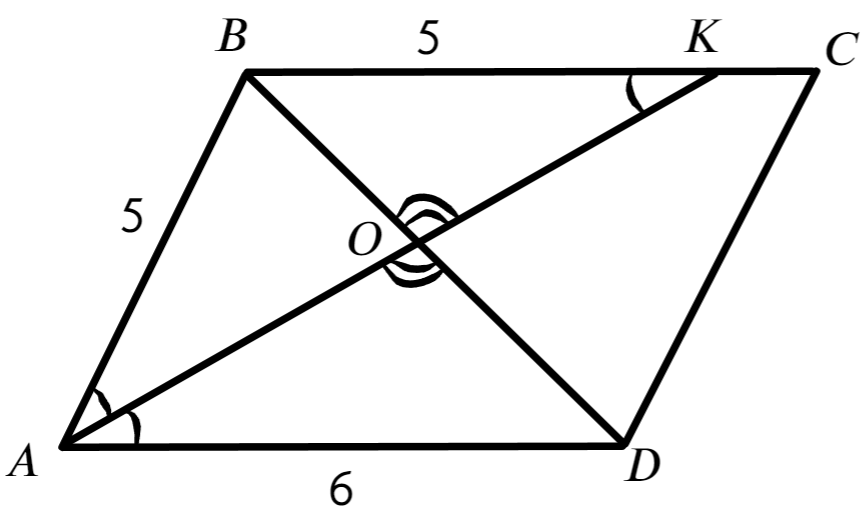
\includegraphics[scale=0.35]{g9-171.png}}
\end{figure}\\
Так как $AK$ --- биссектриса, а углы $BKO$ и $OAD$ являются накрест лежащими при параллельных прямых $AD$ и $BC,$ имеем равенства $\angle BAK=\angle OAD=\angle BKA,$ поэтому треугольник $ABK$ является равнобедренным и $BK=AB=5.$ $\angle BOK=\angle AOD$ как вертикальные, а $\angle BKO=\angle OAD$ как накрест лежащие, значит треугольники $BOK$ и $AOD$ подобны (по двум углам) с коэффициентом $\cfrac{BK}{AD}=\cfrac{5}{6}.$ Высота параллелограмма, проведённая к $AD,$ равна $\cfrac{22}{6}=\cfrac{11}{3}.$ Если высота треугольника $BOK$ равна $x,$ то высота треугольника $AOD$ равна $\cfrac{6}{5}x$ и $x+\cfrac{6}{5}x=\cfrac{11}{3},\ \cfrac{11}{5} x=\cfrac{11}{3},\ x=\cfrac{5}{3}.$ Тогда $S_{\Delta BOK}=\cfrac{1}{2}\cdot\cfrac{5}{3}\cdot5=\cfrac{25}{6}.$\\
